\centering
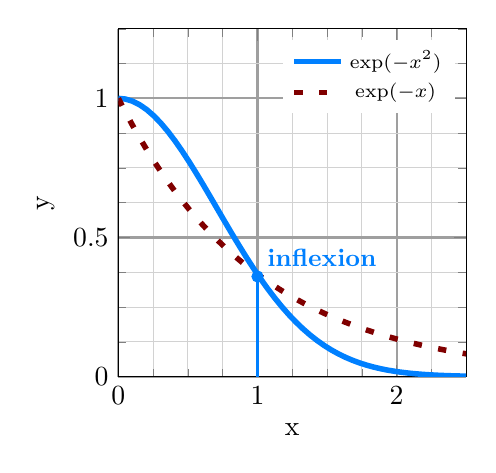
\begin{tikzpicture}[scale=1]
	\begin{axis}[
			height			=	6cm							,
			width			=	6cm							,
			xlabel			=	{x}							,
			ylabel			=	{y}							,
			xmin			=	0    						,
			xmax			=	2.5							,
			ymin			=	0							,
			ymax			=	1.25						,
			legend entries	=	{$\exp(-x^2)$, $\exp(-x)$}	,
			legend style	=	{draw = none, font = \scriptsize}	,
			legend pos		=	north east					,
		    grid 			=   both						,
		    minor tick num 	= 	3 							,
		    minor grid style=   {draw=gray!35} 				,
		    major grid style=   {thick,draw=gray!75} 		,
			]
			
		\addplot[
			color 			=	blue!50!cyan				,
			line width		=	2pt							,
			samples 		= 	50 						,
			domain 			= 	0:2.5						,
			]
			{exp(-x^2)};
			
		\addplot[
			color 			=	red!50!black				,
			line width		=	2pt							,
			samples 		= 	50 							,
			domain 			= 	0:2.5    					,
			loosely dashed									,
			]
			{exp(-x)};
			
		\draw[thick, color = blue!50!cyan] (1,0) -- (1,0.36);
		\addplot[
			mark=*,
			mark options={fill=blue!50!cyan,draw=blue!50!cyan},
			only marks
			]
			coordinates {(1,0.36)};

		% Annotation du point d'inflexion
		\node[anchor=south west, color = blue!50!cyan] at (axis cs:1,0.36) 
		    {\small \bf{inflexion}};
			
	\end{axis}
\end{tikzpicture}
